\documentclass[article]{aaltoseries}
\usepackage[utf8]{inputenc}
\usepackage{url}


\begin{document}
 
%=========================================================

\title{Digital Twins for Industrial Edge 4.0: Concepts and Tools}

\author{Adika Bintang Sulaeman% Your first and last name: do _not_ add your student number
\\\textnormal{\texttt{adika.sulaeman@aalto.fi}}} % Your Aalto e-mail address

\affiliation{\textbf{Tutor}: Prof. Hong-Linh Truong} % First and last name of your tutor

\maketitle

%==========================================================

\begin{abstract}
  Industry 4.0 is expected to be the next big phase in industry. Digital Twins (DT), defined as digital representations of physical objects such as machines, have an important role in Industry 4.0. This paper discusses the digital twin in the context of Industry 4.0 as well as the supporting technologies for digital twins such as the Internet of Things (IoT), cloud computing, fog and edge computing, as well as the software architecture for DT.
  
\vspace{3mm}
\noindent KEYWORDS: Digital Twin, Industrial Internet of Things, Industry 4.0

\end{abstract}


%============================================================


\section{Introduction}

Industry 4.0 is the next big phase in industry. With Industry 4.0, it is possible to gather real-time data from the machines that run in industry and process the data into something meaningful and useful. Industry 4.0 mainly consists of three supporting technologies: IoT, Cyber-Physical Systems (CPS), and Smart Factories \cite{hermann2016design}. The combination of these technologies builds interconnected devices forming Digital Twins (DT).

A DT models a physical object by creating a digital representation using real-time data \cite{Cheatshe3:online}. The data is gathered throughout its life-cycle and used as the source to monitor, learn from, and enhance decision making. A DT enables engineers to monitor and understand how the machines behave once it is released and run by users. Furthermore, engineers can analyze the data and predict the future performance of the machines.

There are some use cases of DT for Industry 4.0. Consider a Printed Circuit Board (PCB) printer for electronic manufacturers. The PCB printer must be very precise, because the smallest error by the laser cutter may lead to PCB flaws. A DT enables engineers and technicians to monitor and analyze the data to predict the time when the spare parts wear out. Another example would be monitoring the jet engine of airplanes. By analyzing data gathered in real-time, engineers and technicians may predict failures in jet systems, which will lead to the reduction of airplane incidents. Furthermore, DT may give feedback to the engineers who design the machine to help them realize an agile development system.

The main value that the DT delivers is an understanding of product performance \cite{Cheatshe3:online}. By understanding performance, manufacturers may detect and understand faults better, create an effective maintenance schedule, troubleshoot machines remotely, and decide appropriate add-on services.

The DT has some challenges in its development and implementation. In \cite{bienhaus2017patterns}, the author has stated a number of challenges such as data consistency between the real physical assets and the digital representation, as well as connectivity and security concerns of cloud computing for DT. Software architectural aspects such as internal structure, APIs, integration, and runtime environment are also critical challenges for DT \cite{malakuti2018architectural}.

\subsection{Scope and Goals}
\label{sec:emphasis}
This paper aims to review the concept of DT for Industry 4.0 as well as the tools and challenges to implement DT in manufacturing context. The role of the IoT, software deployment technologies, API, and cloud computing in DT will be the main focus of this paper. Furthermore, existing approaches in developing and implementing the DTn will also be discussed.

\subsection{Structure}
\label{sec:em}
The rest of this paper is organized as follows. Section 2 discusses the technologies enabling DT. Section 3 discusses the existing approaches and future works. Section 4 concludes this review paper.
 

%============================================================



%============================================================

\section{Key Technologies for Digital Twins}
The entity of DT elements can be modeled as a five-dimension DT \cite{Tao2019}. The five-dimension model consists of Physical Entity (PE), Virtual Entity (VE), Services (SS), DT Data (DD) and Connection (CN). Each of these components require technologies to implement in order to form DT.

\subsection{Physical Entity (PE)}
PE is the real physical entity in the physical space. It contains the real machines with their sensors and actuators. The sensors attached on the PE capture the data from PE during its operation.

To enable PE as DT elements, some technologies are needed. First of all, embedded system is needed on every PE. The computing capabilities embedded in PE is used for reading the data from the sensors and format the data before sent to other DT elements. Secondly, Wireless Sensor Network (WSN) technologies is the backbone of the communication of the sensors data. Other relevant technologies such as distributed sensor layout optimization to reduce redundancy of sensor data, soft sensor to calculate PE's partial parameters, and RFID to track and identify the PE have important role in DT.

\subsection{Virtual Entity (VE)}
VE consists of a set of models representing the PE. Modeling techniques such as three-dimension solid modeling, physics modeling, behavior modeling, and rule modeling are needed to create a useful modeling of the PE. To keep PE and VE model consistent, model consistency analysis, verification, validation and accreditation must be implemented. These techniques may form a solid representation models of the PE. The models can be combined with Virtual Reality (VR) and Augmented Reality (AR) to create the similar environment to the physical space.

\subsection{Services (Ss)}
The software services of the DT is intended to be consumed by PE and VE. The services used by PE includes monitoring service, state prediction service and energy consumption optimization service. VE uses the construction service, calibration service and test service for models.

There are some aspects that need to consider to develop services for modeling DT. Resource management for collecting, classifying, and organizing resources in the DT is an important aspect for the services. The services must also be able to transform resources into software services through digital services. Fault-tolerant management is also important to mitigate failures caused by networks, services, sudden high demands of applications. Human-machine interface is also important to enable interaction between users and services.

\subsection{DT Data (DD)}
DD have data from physical and virtual parts. Therefore, there are massive amount of heterogeneous data. Technologies for processing and securing data including data storage, data modeling, data transformation, data cleaning, data analysis, data mining, data integrity check and data security are required in helping modeling DT data.

\subsection{Connection (CN)}
CN connects different elements of DT. It enables PE, VE, Ss, and DD to communicate to each other. Key technologies of CN includes communication protocol analysis, communication protocol/interface conversion, wireless communication, Application Programming Interface (API) design, as well as communication standard and specification.

\section{Digital Twins Frameworks}
Several researchers have proposed frameworks for implementing DT. This section discusses and analyzes the approaches proposed by researchers.

\subsection{Current Works}
Yu Zheng et. al. proposed an application framework of DT to realize full-physical system mapping, life-cycle dynamic modeling and the whole process real-time optimization \cite{zheng2019application}. This application framework consists of three elements, i.e., physical space, virtual space and information-processing layer. Fig.~\ref{fig:app_framwork_zheng} shows the application framework and the interaction among the physical space, virtual space and information-processing layer.

\begin{figure}[t!]
	\begin{center}
		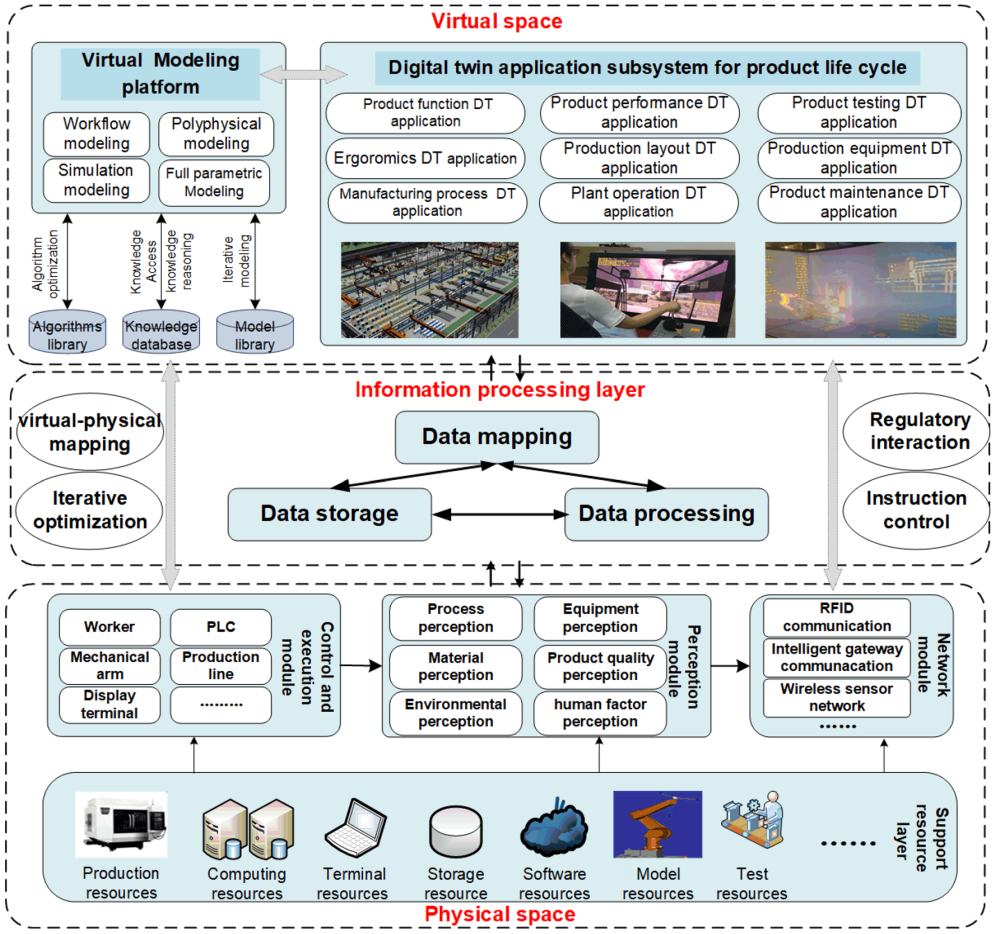
\includegraphics[width=1\textwidth]{figures/app_framework_yu_zheng_et_al}
		\caption{Application Framework for DT \cite{zheng2019application}}
		\label{fig:app_framwork_zheng}
	\end{center}
\end{figure}

The physical space of the framework consists of human workers, machines, materials, rules, and environment. These complex and diverse objects are connected by IoT or WSN technologies. In a manufacturing workshop, for example, sensors and communication equipment collect and deliver data from the physical space such as equipment attributes, status, process, fault and error. Mechanisms and techniques for mapping data to devices are needed to infer the interaction between the physical and digital space.

The information processing layer connects the physical space to virtual space. In addition, it provides bidirectional mapping between physical and virtual space. This layer consists of data storage, data processing, and data mapping modules. Data storage module stores all the data from both physical and virtual space. Data processing module deals with data acquisition, data processing, data analysis, and data fusion. Data mapping utilizes data from storage and processing module to map the operation of physical to virtual space and vice versa.

The virtual space consists of the Virtual Environment Platform (VMP) and DT application subsystem for product lifecycle management. The VMP models 3D virtual model as well as provides operating environment for DT related algorithms. VMP provides virtual models by obtaining data from the database. The data generated from the virtual space is stored as historical data in the database. The combination of historical and real-time data drive the DT application subsystems work synchronously.


\section{Technologies for Digital Twins}
\subsection{Edge Computing, Fog Computing and Cloud Computing Integration for Digital Twins}
Digital Twins and CPS can be divided into three levels according to location of the services: unit level, system level, and System of System (SoS) level \cite{qi2018modeling}. Unit level is the level where local data processing is done by the CPS. The concept of production line, smart factory, and shop floor lies on system level. SoS level is the level which integrates the different systems from system level. Edge computing, fog computing and cloud computing may help integrate the three levels of Digital Twin Systems.

Edge devices, such as the computing resources of the CPS itself, is the source of data. Those devices may also be able to do computation without having to send the data to remote location to reduce latency. Edge computing operation does not always rely on network connection to operate. Therefore, hard real-time response is possible if the computation is done on the edge.

System level may take benefits of fog computing. Fog computing brings the concept of bringing programs to the data, and not vice versa. Fog computing does the computation and storage to the edge network. In this way, the long latency processing that usually comes with cloud computing can be avoided. Human-machine interface and information management systems such as Customer Relationship Management (CRM) cab be connected to the fog computing. However, the capability of devices in fog computing is limited compared to the cloud computing devices. Therefore, at some point, the processing must be done on cloud platform. 

Cloud platform may help digital twin systems in integrating the systems from the system level. Long-term and massive data storage is handled by cloud computing. It provides architectural flexibility and utilization of external parties to be involved in further value creation.

This system architecture has some challenges that needs to be solved. The number of edge and fog devices deployed must be increased. Furthermore, their processing power and storage capacities must be improved to handle more computation. As the computation is done physically close to the users, the security of this systems also require further research.

\subsection{Cloud Technologies for Digital Twins}
Digital twins may take advantages of cloud technologies. The digital twin can be modeled as a Digital Twin-as-a-Service (DTaaS) \cite{borodulin2017towards}. In DTaaS, the cloud platform has a number of levels of abstractions. 

The first level is the digital twin users, who perceive the digital twins as a software service. At the level of the digital twin developer, the cloud platform provides the resources for the development of digital twins as a Platform-as-a-Service (PaaS) model. One of the resources needed by the developers is computing services for specific data operation. These computing services are represented as microservices provided by computing service developers. The computing services are run on a containers provided by the cloud infrastructure providers.

Ciavotta et. al. \cite{ciavotta2017microservice} proposed a microservice-based middleware for digital factory with digital interface in it, named MAYA Platform. The digital interface in that digital factory refers to the digital twin. The designed middleware focuses on enabling interoperability between enterprise applications and CPS.

MAYA Platform is a distributed platform consisting of three main components: MAYA Communication Layer (MCL) for aggregation, discovery, orchestration and communication among CPSs; MAYA Support Infrastructure (MSI) for managing the Digital Twins, enabling definition, data processing, and dismissal with miroservice and Big Data technologies; MAYA Simulation Framework (MSF) for simulation and real-to-digital synchronization of the Digital Twins.

The usage scenario of MAYA Platform can be described as the following:
\begin{itemize}
	\item New CPS devices are registered manually.
	\item The CPS logs in on MSI.
	\item MAYA Platform sets up the Digital Twin Functional Model
	\item The communication is established between CPS and MSI. The CPS sends data to the platform.
	\item The Functional Model creates updates periodically of the corresponding Digital Twin.
	\item The MSF performs the simulation by accessing the simulation model of the Digital Twin.
\end{itemize}

The key focus of the MAYA Platform design is on the MSI. The authors chose microservices because it provides agility, isolation, resilience and elasticity. However, the author also mentioned about the challenges of microservice for this platform, i.e, the difficulties of managing distributed data and the increasing complexity of the software system. Big Data is also part of the MSI. The platform may take benefits of Big Data technologies such as simple but reliable processing, multi-paradigm and general purpose, robust, and scalable.

\subsection{Software Architecture}
Software Web Services and Augmented Reality (AR) may help in visualizing the Digital Twins \cite{schroeder2016visualising}. Data gathered from CPS is stored in data repositories. Web services are implemented to retrieve the data from the repositories, and the data is visualized using AR.

The architecture of the software for Digital Twins visualization can be divided into five layers. The first layer is the device layer, which is a software layer composed by the devices, such as computers, tablets and mobile devices, accessing the system to see the visualization. The second layer is the user interface layer, which can be an AR interface. The third layer is the web service layer using RESTful web service. The forth layer is the query layer, which is responsible for retrieving the data from the data repositories. Finally, the fifth layer is the data repository layer.

\subsection{Big Data and Digital Twins}
Digital Twins' data sources are generated from the product lifecycle in manufacturing such as equipment data, material data, and environmental data collected by IoT \cite{TAO2019183}. The data from the manufacturing process can be high in volume, variety, velocity, variability, and value.

Big data and digital twins can work together to help product design driven development. Without big data and digital twins, some components of manufacturing machines must be manufactured to assess the design quality. Big data and digital twins can create vivid simulations to assess design quality. Big data technologies will process the data from the simulation to identify problems and improve design scheme. The combination of digital twins and big data shortens the design cycle of a product, thus reducing the cost of time and money.



%============================================================


\section{Conclusion}

To be added.


%============================================================


\bibliographystyle{plain}
\bibliography{cs-seminar}

\end{document}
